\section{Geometrie}

% \begin{tabular}{ll c ll c ll}
%     Krümmungskreis-Radius       & S. 254    & & Bogenlänge                  & S. 514    & & Rotations-Oberfläche    & S. 515    \\
%     Krümmungskreis-Mittelpunkt  & S. 255    & & Flächeininhalt              & S. 514    & & Rotations-Volumen       & S. 515    \\
%     Krümmung                    & S. 253 ff       	
% \end{tabular}


\subsection{Kurvendarstellungen}

\textbf{Hinweis: Bei allen Formen muss der Definitionsbereich angegeben werden!}


\begin{minipage}[t]{0.48\columnwidth}
    \subsubsection*{Explizit (2D)}

    \begin{itemize}
        \item Eliminazione parametro $t$ (kann Schwierig sein)
        \item \textbf{Eindeutige} Funktionsgleichung $y = f(x)$
        \item Umkehrfunktion: $x = f^{-1}(y)$
    \end{itemize}
\end{minipage}
\hfill
\begin{minipage}[t]{0.48\columnwidth}
    \subsubsection*{Implizit (2D)}

    \begin{itemize}
        \item $F(x, y) = 0$
        \item nicht eindeutige Gleichung in $x$ und $y$ \\
            z.B. $x^2 + y^2 = 1$
    \end{itemize}
\end{minipage}

\medskip

\begin{minipage}[t]{0.48\columnwidth}
    \subsubsection*{Parameterdarstellung}

    \begin{itemize}
        \item Darstellung als Vektor: $\begin{pmatrix} x(t) \\ y(t) \\ \dots \end{pmatrix}$
        \item $\vec{c}$ ableitbar nach $t$ (keine Knicke)
        \item $\vec{c}$ ist regulär, wenn ableitbar und $\vec{c'} \neq \vec{0}$ (mai $v=0$)
    \end{itemize}
\end{minipage}
\hfill
\begin{minipage}[t]{0.48\columnwidth}
    \subsubsection*{Polarform}

    \begin{itemize}
        \item Darstellung: Radius als Funktion des Winkels:  $r = f(\varphi)$
        \item Darstellung als Polar-Vektor: $\vec{c}(\varphi) = \begin{pmatrix} r(\varphi) \, \cos(\varphi) \\ r(\varphi) \, \sin(\varphi) \end{pmatrix}$
        \item Im Pol bedeutet $r = 0$ ; Winkel $\varphi_0$ z.B. $\pi$
        \item Drehung um Winkel $\alpha$: $r(\varphi) \rightarrow r(\varphi - \alpha)$ \\
            (Drehung  im Gegenuhrzeigersinn)
    \end{itemize}
\end{minipage}

\medskip

\begin{minipage}[t]{0.48\columnwidth}
    \subsubsection*{Tangentialvektor}

    \begin{itemize}
        \item Vettore di velocità istantanea
        \item Darstellung als Vektor: $\frac{\diff}{\diff t}\vec{c} =  \begin{pmatrix} \dot{x}(t) \\ \dot{y}(t) \\ \dots \end{pmatrix}$
        \item Punkt steht für Ableitung nach der Zeit
    \end{itemize}
\end{minipage}
\hfill
\begin{minipage}[t]{0.48\columnwidth}

\end{minipage}



\subsection[Polarkoordinaten]{Polarkoordinaten $\bm{(r, \, \varphi)}$}{197-198}

\vspace{-0.2cm}

\[ r = \sqrt{x^2 + y^2} \qquad \qquad 
x = r \cdot \cos(\varphi) \qquad \qquad 
y = r \cdot \sin(\varphi) \qquad \qquad 
\varphi = \begin{cases}			
    \arctan \big( \frac{y}{x} \big)         & x > 0 \\
    \arctan \big( \frac{y}{x} \big) + \pi   & x < 0 \\
    \frac{\pi}{2}                           & x = 0 \wedge y > 0\\
    -\frac{\pi}{2}                           & x = 0 \wedge y < 0\\
\end{cases} \]


\[ \text{Polar-Vektor:} \quad \vec{c}(\varphi) = 
\begin{pmatrix} r(\varphi) \, \cos(\varphi) \\ 
r(\varphi) \, \sin(\varphi) \end{pmatrix} \qquad 
 \text{ \textrightarrow\ } r \text{ ist eine Funktion des Winkels } \varphi \]

\subsection{Umrechnung Darstellungsformen (Koordinatensysteme)}

\renewcommand{\arraystretch}{1.2}
\begin{ctabular}{lcl l}
    \toprule
    Parameter       & \textrightarrow\  & Explizit  & $t$ eliminieren; ineinander einsetzen; umformen                                                   \\
    \midrule
    Ex- / Implizit  & \textrightarrow\  & Polar     & Ersetzen: $x = r \cdot \cos(\varphi) \quad y = r \cdot \sin(\varphi) \quad x^2 + y^2 = r^2$       \\
    \midrule
    Polar           & \textrightarrow\  & Implizit  & Ersetzen: $r \cdot \cos(\varphi) = x \quad r \cdot \sin(\varphi) = y \quad r = \sqrt{x^2 + y^2}$  \\
    \midrule
    Polar           & \textrightarrow\  & Parameter &   $\begin{pmatrix}    r(\varphi) \cdot \cos(\varphi) \\
                                                                            r(\varphi) \cdot \sin(\varphi) \end{pmatrix} = 
                                                        \begin{pmatrix}     x(\varphi) \\ 
                                                                            y(\varphi) \end{pmatrix}$                                                   \\
    \midrule
    Explizit        & \textrightarrow\  & Parameter & $\begin{pmatrix} x \\ f(x) \end{pmatrix} = \begin{pmatrix} x(t) \\ y(t) \end{pmatrix}$            \\
    \bottomrule
\end{ctabular}
\renewcommand{\arraystretch}{1}

\subsubsection{Dominio di $\varphi$}
\begin{enumerate}
    \item \textbf{Esistenza Algebrica}: Denominatori $\neq 0$ e argomenti delle radici $\ge 0$.
    \item \textbf{Positività del Raggio}: Poiché $r$ è una distanza, imponi $r(\varphi) \ge 0$.
    \[ f(\varphi) \ge 0 \qquad \text{(Nominatore e Denominatore con lo stesso segno)}\]
    \item \textbf{Vincolo Arcotangente}: Se $\varphi = \arctan(y/x)$, allora:
    \[ \varphi \in \left( -\frac{\pi}{2}, \frac{\pi}{2} \right)\]
    \item \textbf{Dominio Finale}: Intersezione di tutti i vincoli sopra indicati.
    \[ \mathcal{D}_{\varphi} = \{ \text{Punti 1} \cap \text{Punti 2} \cap \text{Punti 3} \} \]
\end{enumerate}

\columnbreak


\subsection{Kreis (Kurve 2. Ordnung)}{204}

\begin{minipage}[c]{0.22\columnwidth}
    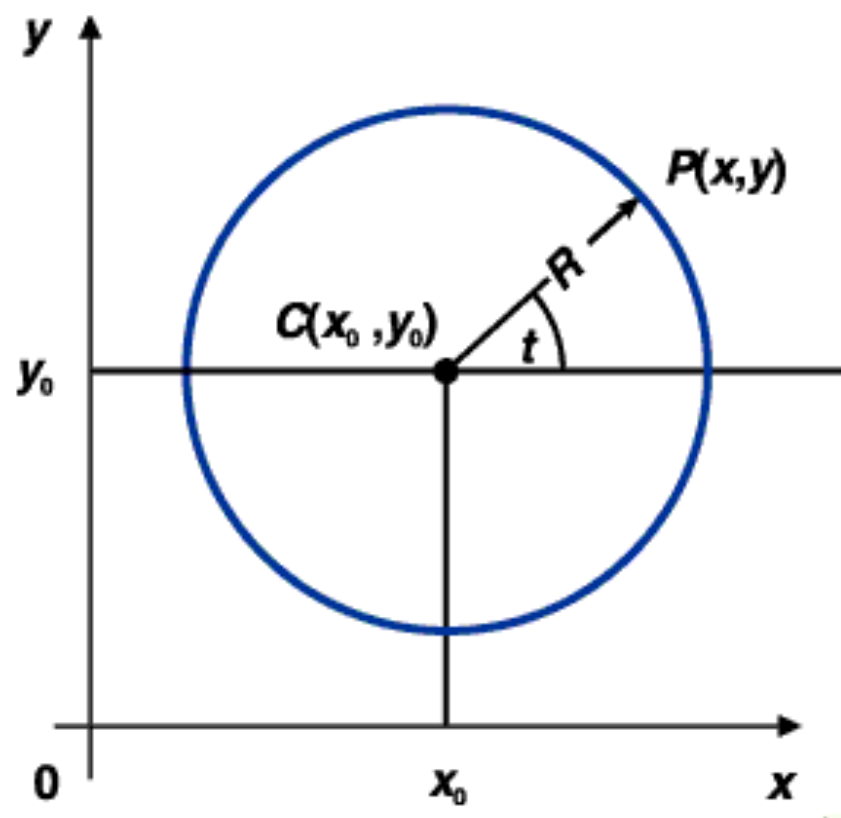
\includegraphics[width=\columnwidth]{images/kreis.png}
\end{minipage}
\hfill
\begin{minipage}[c]{0.77\columnwidth}
    \begin{tabular}{lll}
        $r$     & Radius (im Folgenden $R$, da konstant)    \\
        $x_0$   & $x$-Koordinate des Kreismittelpunktes     \\
        $y_0$   & $y$-Koordinate des Kreismittelpunktes
    \end{tabular} 

    
    \begin{ctabular}{ l  c  c  c }
        \toprule
                & Implizit                          & Paramter (Vektor)                                                                                                             & Polar                     \\
                & (Achsenkreuz in $O$)              & (Achsenkreuz in $O$)                                                                                                          & (Achsenkreuz in $O$)      \\
        \midrule
        Kurve   & $(x - x_0)^2+ (y - y_0)^2 = R^2$  & $\begin{pmatrix} x(t) \\ y(t) \end{pmatrix} = \begin{pmatrix} x_0 + R \cdot \cos(t) \\ y_0 + R \cdot \sin(t) \end{pmatrix}$   & $r(\varphi) = R$ (const)  \\
        \bottomrule
    \end{ctabular}
\end{minipage}


% \begin{tabular}{| l | c | c | c |}
%     \hline
%             & Implizit                          & Paramter (Vektor)                                                                                                             & Polar                     \\
%             & (Achsenkreuz in $O$)              & (Achsenkreuz in $O$)                                                                                                          & (Achsenkreuz in $O$)      \\
%     \hline
%     Kurve   & $(x - x_0)^2+ (y - y_0)^2 = R^2$  & $\begin{pmatrix} x(t) \\ y(t) \end{pmatrix} = \begin{pmatrix} x_0 + R \cdot \cos(t) \\ y_0 + R \cdot \sin(t) \end{pmatrix}$   & $r(\varphi) = R$ (const)  \\
%     \hline
% \end{tabular}



\subsection{Ellipse (Kurve 2. Ordnung)}{205}

\begin{minipage}[c]{0.38\columnwidth}
    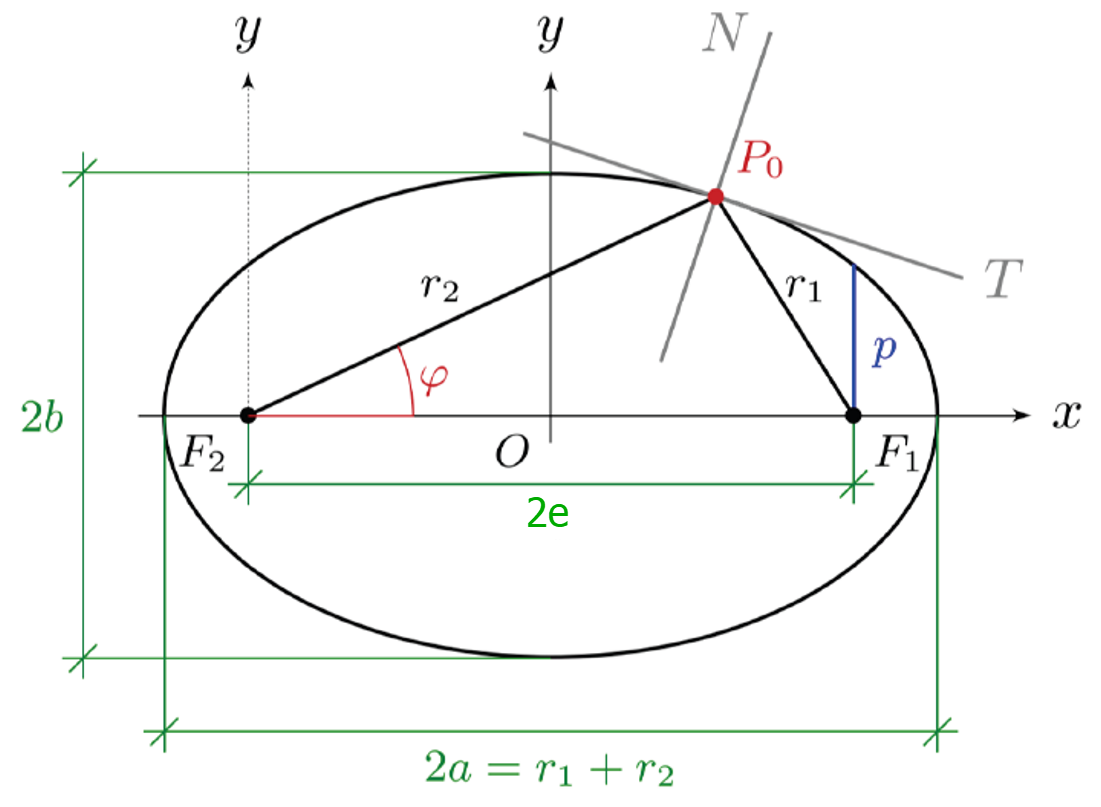
\includegraphics[width=\columnwidth]{images/ellipse.PNG}
\end{minipage}
\hfill
\begin{minipage}[c]{0.58\columnwidth}
    \renewcommand{\arraystretch}{1.3}
    \begin{tabular}{lll}
        $a$             & Grosse Halbachse (horizontal) & $a = \frac{p}{1-\varepsilon^2}$                                                             \\
        $b$             & Kleine Halbachse (vertikal)   &                                                                  \\
        $e$             & Extrentrizität                & $e = \sqrt{a^2 - b^2}$                                        \\
        $\varepsilon$   & num. Exzentrizität            & $\varepsilon = \frac{e}{a} \quad $\colorbox{yellow}{$(0 \leq \varepsilon < 1)$}    \\
        $p$             & Halbparameter                 & $p =\frac{b^2}{a}$                                            \\
                        & (leggibile direttamente da asse $y$) & \\
        $\varphi$       & Polarwinkel bei $F_2$         & $0 \leq \varphi < 2 \pi$ 	                                    \\
        $F_1, \, F_2$   & Brennpunkte                                                                                   \\
        $r_1, \, r_2$   & Polabstände zu $F_{1,2}$
    \end{tabular}
    \renewcommand{\arraystretch}{1}
\end{minipage}

\renewcommand{\arraystretch}{1.4} % Aumentato per ospitare meglio le frazioni in \displaystyle
\begin{ctabular}{l c cc cc}
    \toprule
    & Implizit & & Parameter (Vektor) & & Polar \\
    & (Achsenkreuz in O) & & (Achsenkreuz in  O) & & \textbf{\color{orange}(Achsenkreuz in $\boldsymbol{F_2}$)} \\
    
    \midrule
    \textbf{Kurve} 
    & $\displaystyle \left( \frac{x}{a} \right)^2 + \left( \frac{y}{b} \right)^2 = 1$ 
    & & $\displaystyle \begin{pmatrix} x(t) \\ y(t) \end{pmatrix} = \begin{pmatrix} a \cdot \cos(t) \\ b \cdot \sin(t) \end{pmatrix}$ 
    & & $\displaystyle r(\varphi) = \frac{p}{1 - \varepsilon \cdot \cos(\varphi)}$ \\
    
    & & & $0 \leq t < 2\pi$ 
    & & $0 < \varphi < 2\pi$ \\
    
    \midrule
    \textbf{Tangentensteigung} 
    & $\displaystyle \frac{\diff y}{\diff x} = \frac{-b^2}{a^2} \cdot \frac{x_0}{y_0}$ 
    & & $\displaystyle \frac{\diff y}{\diff x} = \frac{\dot{y}_0(t)}{\dot{x}_0(t)} = \frac{b \cdot \cos(t_0)}{-a \cdot \sin(t_0)}$ 
    & & $\displaystyle \frac{\diff y}{\diff x} = \frac{\dot{y}(t)}{\dot{x}(t)} = \frac{\varepsilon - \cos(\varphi)}{\sin(\varphi)}$ \\
    
    & & & & & $\varphi \neq 0, \, \pi$ \\
    
    $(x_0, y_0) = P_0$ 
    & $y_0 \neq 0$ 
    & & $t \neq 0, \, \pi$ 
    & & $\text{AP: } (x_0; \, y_0) = \begin{pmatrix} r_0 \cdot \cos(\varphi_0) \\ r_0 \cdot \sin(\varphi_0) \end{pmatrix}$ \\
    \bottomrule
\end{ctabular}

Come si può notare (asse $y$ tratteggiato), la rappresentazione polare ha l'origine
posta nel fuoco $F_2$ .Per riportare la curva nel sistema cartesiano (centrato in O),
è necessaria una \textbf{traslazione di $e$ lungo l'asse $x$} \textrightarrow $(\frac{x-e}{a})^2 + \dots$.

\subsection{Kardioide (Kurve 2. Ordnung)}{100}	

\begin{minipage}[t]{0.26\columnwidth}
    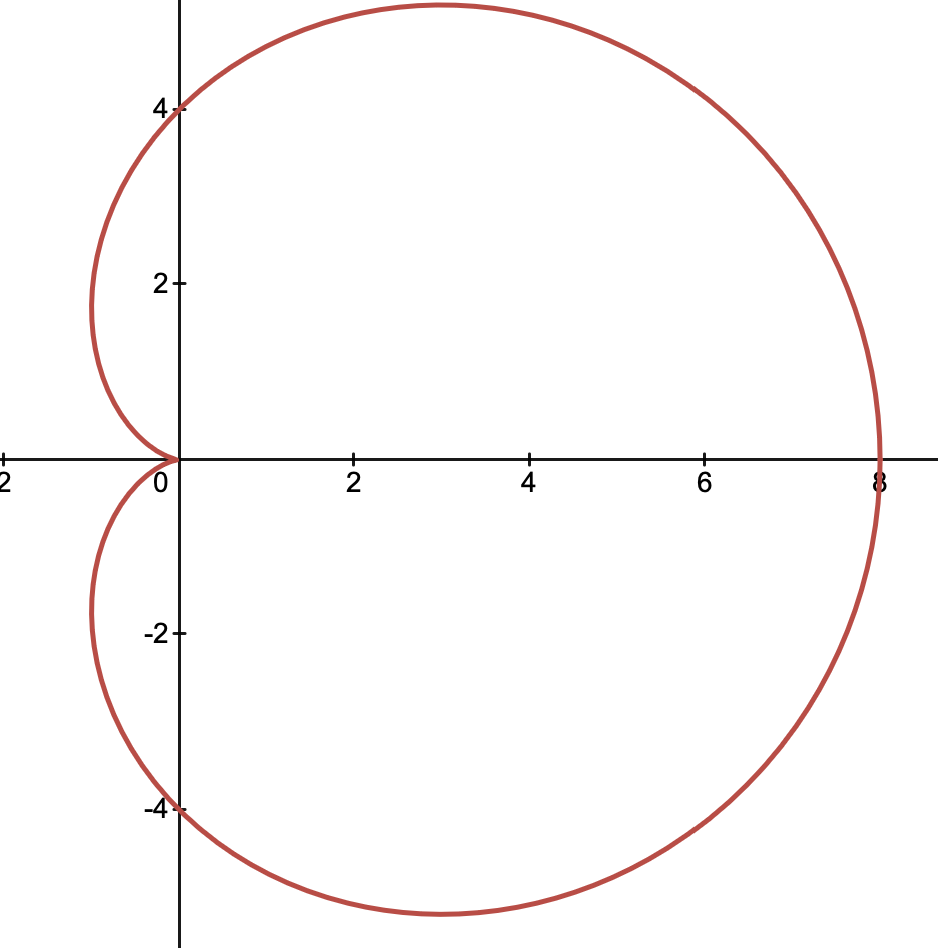
\includegraphics[width=\linewidth, align=t]{images/kardioide.PNG}
\end{minipage}
\hfill
\begin{minipage}[t]{0.72\columnwidth}
    Allgemein gilt für Limaçons die Darstellung $r = f(\varphi)$ mit Pol bei $r = 0$

    \medskip

    \begin{tabular}{ll}
        $a$ & Streckfaktor zum Pol 
    \end{tabular} 
    
    \begin{ctabular}{l c cc cc }
        \toprule
                & Implizit              & & Paramter (Vektor)                                                                                                                                         & & Polar                                                 \\
                &                       & & (Achsenkreuz in $O$)                                                                                                                                      & & (Achsenkreuz in $O$)                                  \\
        \midrule
        Kurve   & --                    & & $\begin{pmatrix} x(t) \\ y(t) \end{pmatrix} = \begin{pmatrix} a \cdot (1 + \cos(t))\cdot \cos(t) \\ a \cdot (1 + \cos(t)) \cdot \sin(t)  \end{pmatrix} $  & & $r(\varphi) = a \cdot \Big(1 + \cos(\varphi) \Big)$   \\
        \bottomrule
    \end{ctabular}
\end{minipage}
\renewcommand{\arraystretch}{1}
    

\subsection{Parabel (Kurve 2. Ordnung)}{210}

\begin{minipage}[c]{0.38\columnwidth}
    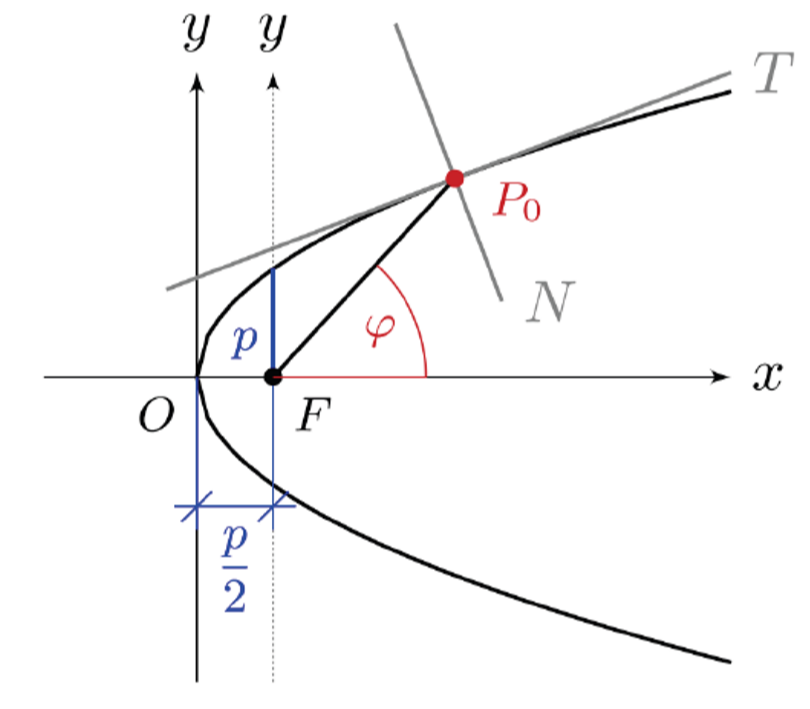
\includegraphics[width=\columnwidth]{images/parabel.PNG}
\end{minipage}
\hfill
\begin{minipage}[c]{0.6\columnwidth}
    \begin{tabular}{lll}
    $\varepsilon$   & num. Exzentrizität    & \colorbox{yellow}{$\varepsilon = 1$}     \\
    $p$             & Halbparameter                                 \\
    $\varphi$       & Polarwinkel           & $0 < \varphi < 2 \pi$ \\
    $F$             & Brennpunkt
    \end{tabular}
\end{minipage}

\begin{ctabular}{l c cc cc}
    \toprule
    & Implizit & & Parameter (Vektor) & & Polar \\
    & (Achsenkreuz in O) & & (Achsenkreuz in O) & & \textbf{(Achsenkreuz in $\boldsymbol{F}$)} \\
    
    \midrule
    \textbf{Kurve} 
    & $\displaystyle y^2 = 2px$ 
    & & $\displaystyle \begin{pmatrix} x(t) \\ y(t) \end{pmatrix} = \begin{pmatrix} \frac{y^2}{2p} \\ y \end{pmatrix}$ 
    & & $\displaystyle r(\varphi) = \frac{p}{1 - \varepsilon \cdot \cos(\varphi)}$ \\
    
    & & & $y \in \mathbb{R}$ 
    & & $(\varepsilon = 1)$ \\
    
    \midrule
    \textbf{Tangentensteigung} 
    & $\displaystyle y' = f(x)' = \frac{p}{y}$ 
    & & $\displaystyle y' = \frac{p}{y}$ 
    & & $\displaystyle y' = \frac{1 - \cos(\varphi)}{\sin(\varphi)}$ \\
    
    & $y \neq 0$; $y = \text{Parabelpunkt}$ 
    & & $y \neq 0, \, y = \text{Parabelpunkt}$ 
    & & $\varphi \neq 0, \, \pi$ \\
    \bottomrule
\end{ctabular}

Per riportare la curva nel sistema cartesiano (centrato in O),
è necessaria una \textbf{traslazione di $\frac{1}{2}p$ entgegen l'asse $x$} \textrightarrow $\dots \cdot (x+\frac{p}{2})$.

\subsection{Hyperbel (Kurve 2. Ordnung)}{207}	

\begin{minipage}{0.34\columnwidth}
    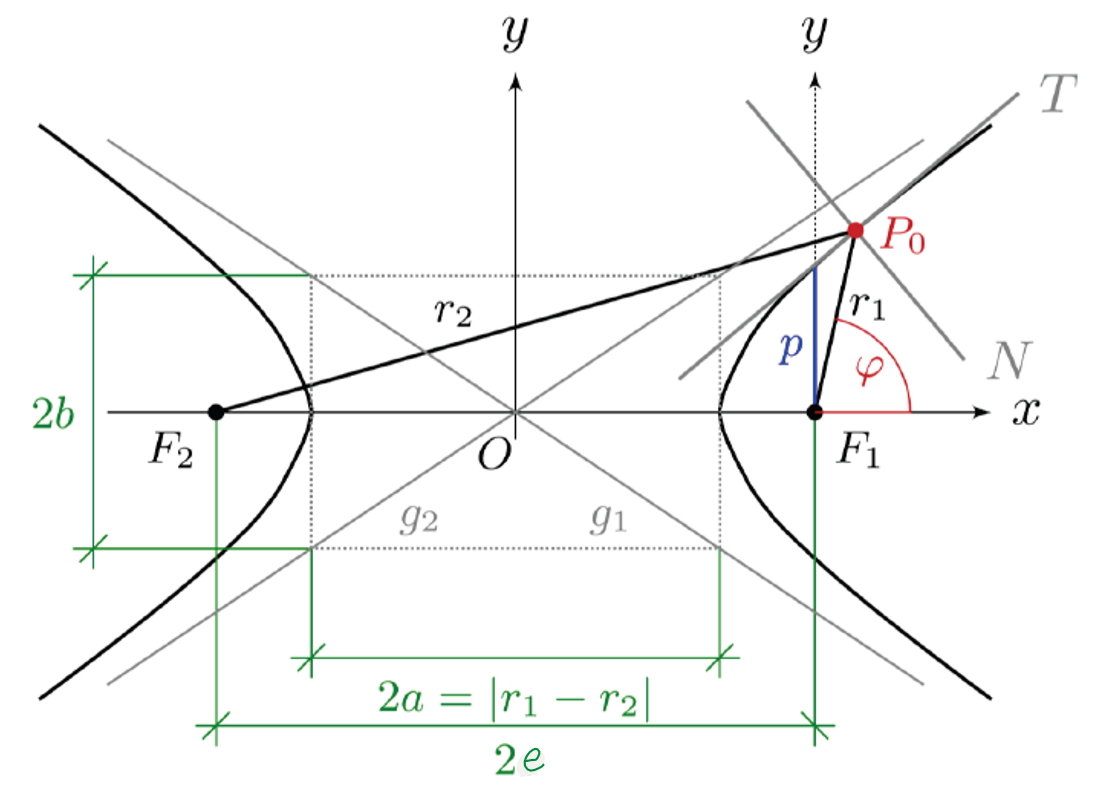
\includegraphics[width=\columnwidth]{images/hyperbel.PNG}
\end{minipage}
\hfill
\begin{minipage}{0.63\columnwidth}
    \renewcommand{\arraystretch}{1.2}
    \begin{tabular}{lll}
        $a$             & Halbachse horizontal                  & $a = \frac{p}{\varepsilon^2 - 1}$                                                                                                                          \\   
        $b$             & Halbachse vertikal                                                                                                                                            \\
        $e$             & Extrentrizität                        & $e = \sqrt{a^2 + b^2}$                                                                                                \\
        $\varepsilon$   & num. Exzentrizität                    & $\varepsilon = \frac{e}{a} \qquad $\colorbox{yellow}{$(\varepsilon > 1)$}                                                   \\
        $p$             & Halbparameter                         & $p =\frac{b^2}{a}$                                                                                                    \\
        $\varphi$       & Polarwinkel bei $F_1$                 & $\varphi \notin \Big[ -\arccos \Big( \frac{1}{\varepsilon} \Big); \, \arccos \Big( \frac{1}{\varepsilon} \Big) \Big]$ \\
        $F_1, \, F_2$   & Brennpunkte                                                                                                                                                   \\
        $r_1, \, r_2$   & Polabstände zu $F_{1,2}$                                                                                                                                      \\
        $g_1, \, g_2$   & Asymptoten; Steigung $\pm \frac{b}{a}$
    \end{tabular}
    \renewcommand{\arraystretch}{1}
\end{minipage}

\begin{ctabular}{l c cc cc}
    \toprule
    & Implizit & & Parameter (Vektor) & & Polar \\
    & (Achsenkreuz in O) & & (Achsenkreuz in O) & & (\textbf{Achsenkreuz in $\boldsymbol{F_1}$}) \\
    
    \midrule
    \textbf{Kurve} 
    & $\displaystyle \left( \frac{x}{a} \right)^2 - \left( \frac{y}{b} \right)^2 = 1$ 
    & & $\displaystyle \begin{pmatrix} x(t) \\ y(t) \end{pmatrix} = \begin{pmatrix} a \cdot \cosh(t) \\ b \cdot \sinh(t) \end{pmatrix}$ 
    & & $\displaystyle r(\varphi) = \frac{p}{1 - \varepsilon \cdot \cos(\varphi)}$ \\
    
    & & & $t \in \mathbb{R}$ ; \textbf{\color{orange}rechter Ast} 
    & & $(\varepsilon > 1)$; \textbf{\color{orange}rechter Ast} \\
    \bottomrule
\end{ctabular}

Per riportare la curva nel sistema cartesiano (centrato in O),
è necessaria una \textbf{traslazione di $e$ entgegen l'asse $x$} \textrightarrow $(\frac{x+e}{a})^2-\dots$.

\subsection{Krümmung}

\vspace{-0.2cm}

\[\text{Krümmung:} \quad \kappa = \frac{\diff \alpha}{\diff s} = \kappa(x_0) \quad (\text{in AP } x_0; \, y_0)\]

\medskip

\begin{minipage}[t]{0.55\columnwidth}
    \renewcommand{\arraystretch}{1.4}
    \begin{tabular}{lllll}
        konkav: & Rechtskurve   & $f''(x) \leq 0$   & $ f' \downarrow$  & $\kappa(x) \leq 0$    \\
        konvex: & Linkskurve    & $f''(x) \geq 0$   & $ f' \uparrow$    & $\kappa(x) \geq 0$    \\
        \\
    \end{tabular}
    \renewcommand{\arraystretch}{1}
\end{minipage}
\hfill
\begin{minipage}[t]{0.44\columnwidth}
    \renewcommand{\arraystretch}{1.4}
    \begin{tabular}{ll}
        Wendepunkt  & $\kappa = 0$ \myul{und} Vorzeichenwechsel         \\
        Scheitel    & $\kappa$ extremal (Minimum; Maximum)              \\
        Flachpunkt  & $\kappa = 0$ \myul{aber} kein Vorzeichenwechsel 
    \end{tabular}
    \renewcommand{\arraystretch}{1}
\end{minipage}



\begin{minipage}[c]{0.68\columnwidth}
    \begin{center}
    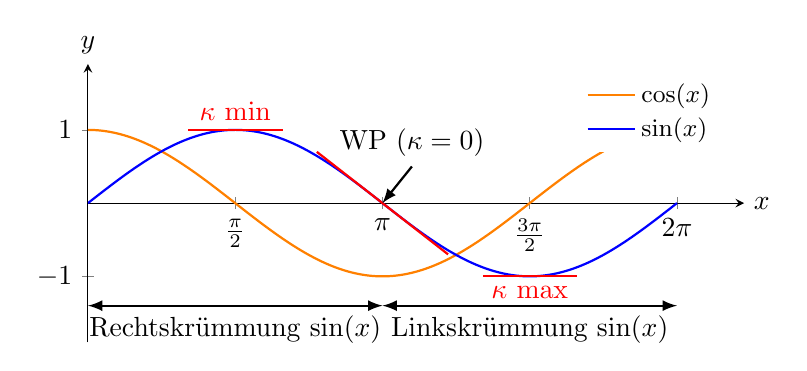
\begin{tikzpicture}
        \begin{axis}[
            scale=0.8,
            >=latex,
            xmin=0,
            xmax=7,
            ymin = -1.9,
            ymax = 1.9,
            width=12cm,
            height=6cm,
            samples=200,      
            axis x line=middle, 
            axis y line=middle, 
            xtick={0, pi/2, pi, 3*pi/2, 2*pi},
            xticklabels={$0$, $\frac{\pi}{2}$, $\pi$, $\frac{3\pi}{2}$, $2\pi$},
            ytick={-1, 0, 1},
            x label style={anchor=west},
            xlabel={$x$}, 
            y label style={anchor=south},
            ylabel={$y$},
            legend pos=north east,
            legend style={font=\small, cells={anchor=west}, draw=none}
        ]
        
        % cos()
        \addplot[orange, thick, domain=0:2*pi] {cos(deg(x))};
        \addlegendentry{$\cos(x)$}

        % sin()
        \addplot[blue, thick, domain=0:2*pi] {sin(deg(x))};
        \addlegendentry{$\sin(x)$}
        
        % Tangenten an sin()
        \addplot[red, thick, domain=pi/2-0.5:pi/2+0.5] {1};
        \node[above, red] at (pi/2, 1) {$\kappa$ min};

        \addplot[red, thick, domain=3*pi/2-0.5:3*pi/2+0.5] {-1};
        \node[below, red] at (3*pi/2, -1) {$\kappa$ max};

        \addplot[red, thick, domain=pi-0.7:pi+0.7] {-(x - 3*pi/2) - pi/2};

        \draw[->, thick] (1.1*pi, 0.5) node[above] {WP $(\kappa = 0)$} -- (pi, 0);

        \draw[<->, thick] (0, -1.4) -- (pi, -1.4) node[below, midway] {Rechtskrümmung $\sin(x)$};

        \draw[<->, thick] (pi, -1.4) -- (2*pi, -1.4) node[below, midway] {Linkskrümmung $\sin(x)$};

        \end{axis}
    \end{tikzpicture}
\end{center}
\end{minipage}		
\hfill
\begin{minipage}[c]{0.3\columnwidth}
    \textbf{Extremalwerte der Krümmung}	

    \smallskip

    \textbf{ \textrightarrow\ Tricks anwenden!}

    \medskip

    \renewcommand{\arraystretch}{1.4}
    \begin{tabular}{ll}
    Maximum:    & simultan $\frac{\text{Zaehler max}}{\text{Nenner min}}$ \\
    Minimum:    & simultan $\frac{\text{Zaehler min}}{\text{Nenner max}}$
    \end{tabular}		
    \renewcommand{\arraystretch}{1}
\end{minipage}		

È anche possibile analizzare lo Scheitel \textit{(vertice)} di una curva analizzando 
la forma (z.B un iperbole ha $s = (\pm a,0)$)

\subsection{Krümmungskreis (Approximation 2. Ordnung)}	

\begin{ctabular}{ll c ll}
    2D & Krümmungs\textbf{kreis} mit Radius $r = \frac{1}{ \vert \kappa \vert }$ & & 
    3D & Krümmungs\textbf{kugel} mit Radius $r = \frac{1}{\vert \kappa \vert }$
\end{ctabular}

\subsubsection{Eigenschaften des Krümmungskreises}

\begin{itemize}
    \item Krümmungskreis hat gleiche Krümmung wie Kurve in Arbeitspunkt
    \item Tangentenrichtung von Krümmungskreis und Kurve sind identisch
    \item Zentrum des Kreises liegt auf der Normalen auf der Seite von $\ddot{\vec{c}}$
\end{itemize}
	

\subsection{Evolute (Kurve der Krümmungskreismittelpunkte)}{262}

\begin{minipage}{0.32\columnwidth}
    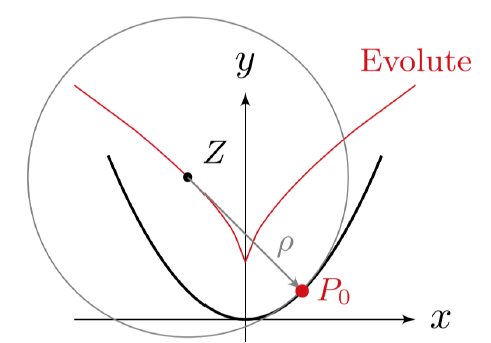
\includegraphics[width=\columnwidth]{images/evolute.PNG}
\end{minipage}
\hfill
\begin{minipage}{0.65\columnwidth}
    \begin{itemize}
        \item Die Evolute beschreibt die Kurve der Krümmungskreismittelpunkte
        \item Die Evolute erfüllt die folgende Vektorgleichung 
    \end{itemize}    

    \[ \begin{pmatrix} x_c \\ y_c \end{pmatrix} = \begin{pmatrix} x \\ y \end{pmatrix} + \frac{1}{\kappa} \, \vec{n} \]
\end{minipage}


\subsubsection{Krümmungskreis-Mittelpunkt}{255}

\renewcommand{\arraystretch}{2}
\begin{ctabular}{ cc cc  cc }
    \toprule
    Explizit                            & & Parameter (Vektor)                                                                        & & Polar                                                                                                                                                         \\
    \midrule
    $x_c = x - \dfrac{y'(1+y'^2)}{y''}$  & & $ x_c(t) = x - \dot{y} \dfrac{\dot{x}^2 + \dot{y}^2}{\dot{x} \ddot{y} - \ddot{x} \dot{y}}$ & & $x_c = r \cdot \cos(\varphi) - \dfrac{\left( r^2  + \dot{r}^2 \right) \cdot \left( r \cdot \cos(\varphi) + \dot{r} \cdot \sin(\varphi) \right) }{r^2 + 2 \dot{r}^2 - r \, \ddot{r}}$ \\
    $y_c = y + \dfrac{1 + y{'} ^2}{y''}$ & & $ y_c(t) = y + \dot{x} \dfrac{\dot{x}^2 + \dot{y}^2}{\dot{x} \ddot{y} - \ddot{x} \dot{y}}$ & & $y_c = r \cdot \sin(\varphi) - \dfrac{\left( r^2  + \dot{r}^2 \right) \cdot \left( r \cdot \sin(\varphi) + \dot{r} \cdot \cos(\varphi)\right) }{r^2 + 2 \dot{r}^2 - r \, \ddot{r}}$ \\
    \bottomrule
\end{ctabular}
\renewcommand{\arraystretch}{1}

\subsection{Kurven Ordnung}
Due curve $f(x)$ e $g(x)$ hanno un contatto di \textbf{ordine $n$} in un punto $x_0$ se tutte le loro derivate fino all'ordine $n$ coincidono in quel punto, ma la derivata $(n+1)$-esima è diversa.

\begin{equation*}
    f^{(k)}(x_0) = g^{(k)}(x_0) \quad \text{per ogni } k = 0, 1, \dots, n
\end{equation*}
\begin{equation*}
    f^{(n+1)}(x_0) \neq g^{(n+1)}(x_0)
\end{equation*}

\subsubsection{Metodi di calcolo veloci}
\begin{itemize}
    \item \textbf{Molteplicità delle radici:} Se l'equazione $f(x) - g(x) = 0$ ha una soluzione in $x_0$ con molteplicità $k$, allora l'ordine di contatto è $n = k - 1$.
    \item \textbf{Sviluppo di Taylor:} Se $g(x)$ è il polinomio di Taylor di grado $n$ della funzione $f(x)$ centrato in $x_0$, allora il contatto tra la funzione e il polinomio è (almeno) di ordine $n$.
\end{itemize}